\section{Aufbau}
\begin{figure}
	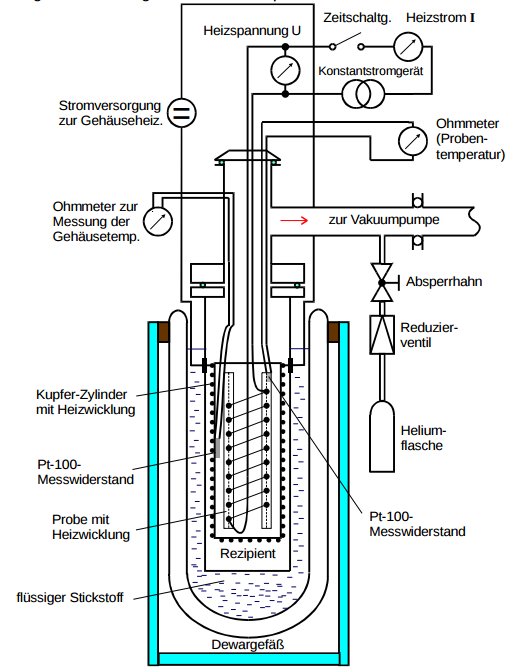
\includegraphics[width=\textwidth, draft, ]{graphics/aufbau.pdf}
	\caption{Skizzenhafter Aufbau des Versuchs. \cite{skript}}
	\label{fig:aufbau}
\end{figure}
In einem Dewar-Gefäß befindet sich der Rezipient; 
darin befinden sich die Kupferprobe, die Messeinrichtung, Druckgasventile und Heizsysteme.
Der Rezipient ist mit Gas befüllbar und kann mittels einer Vakuumpumpe evakuiert werden. 
Sowohl die Kupferprobe als auch das Gehäuse des Rezipienten sind mit unabhängigen Heizungen ausgestattet.
Die Messeinrichtung besteht aus zwei Pt-100-Messwiderständen, 
je eine an beiden Heizungen, 
sodass die Temperaturen und Heizleistung beobachtet werden können.
Der Versuchsaufbau ist in \ref{fig:aufbau} dargestellt.


\section{Durchführung}
Es wird die Temperatur-Abhängigkeit der Molwärme $C_\text{p}$ von Kupfer im
Bereich von $\SI{80}{\kelvin}$ bis $\SI{300}{\kelvin}$ gemessen. 
Zum Kühlen der Probe wird der Rezipient mit gasförmigen Helium bei Barometerdruck geflutet 
und das Dewar-Gefäß mit flüssigem Stickstoff gefüllt.
Erreichen sowohl Gehäuse als auch die Probe die gleiche minimale Temperatur, 
wird mittels der Vakuumpumpe der Rezipient evakuiert und der Druck bis zum Ende der Messungen kleinstmöglich gehalten.
Über die Probenheizung kann der Probe Wärme zugeführt werden, 
während die davon unabhängige Heizung die Gehäusetemperatur auf Probentemperatur hält.
Es wird die Probenheizspannung $U$, Probenheizstrom $I$ und die Zeit $t$ in Abschnitten notiert, 
in welchen die Probe um $\SI{11}{\kelvin}$ erwärmt wird.